%!TEX program = xelatex
\documentclass[11pt, a4paper]{scrartcl}
%\documentclass[11pt, a4paper]{article}
\usepackage[utf8]{inputenc}
%\usepackage[a4paper,lmargin={3.5cm},rmargin={3.5cm}, tmargin={2.5cm},bmargin = {2.5cm}]{geometry}
\usepackage{setspace}
\usepackage{indentfirst}
\usepackage{mathtools}
\usepackage{enumitem}
\usepackage{graphicx}
\usepackage{amsmath, amssymb}
\usepackage[backend=biber, authordate, ibidtracker=context]{biblatex-chicago}
\usepackage{titlesec}
\usepackage{color}

\onehalfspacing{}
\addbibresource{conceptsimilarity.bib}

\usepackage{fontspec}
\newfontfamily\osfamily{Latin Modern Roman Demi}

\setkomafont{disposition}{\osfamily}


\renewcommand{\i}[1]{\emph{#1}}
\renewcommand{\L}{\mathcal{L}}
\newcommand{\given}[1][]{\:#1\vert\:}

\titleformat{\section}{\Large\bfseries\osfamily}{\thesection}{1em}{}
\titleformat{\subsection}{\large\bfseries\osfamily}{\thesubsection}{1em}{}

\title{\osfamily\textbf{Meaning as Conceptual Role}\\ in a Spatial Interpretation}
\author{Class Paper for Logic and Probability \\ Prof.\ Dr.\ Hannes Leitgeb \\ SS2017, LMU Munich \\ Conrad Friedrich \\ \texttt{conradfriedrich@posteo.net}}

\begin{document}

\maketitle
\abstract{This paper tries to answer the question what can be said regarding the semantic meaning of a linguistic expression when all that is given is a set of sentences and a subjective probability function, ingredients standardly assumed in formal epistemology. We take a look at several approaches to explicate meaning using spatial metaphors, combining favorable aspects to present an account of similarity in conceptual role based on a spatial interpretation of conditional probabilities.}
\thispagestyle{empty}
\newpage
\tableofcontents
\newpage
\section{Introduction}

\subsection{Field's Notion of Conceptual Role}
\subsection{Gärdenfors' Conceptual Spaces}
Gärdenfors' Dimensions are rooted in phenomenal experiences and mostly are motivated by empirical, psychological research.
\subsection{Word Space Models in Computational Linguistics}
Its seems like a very natural idea: The geometric interpretation of mental representations provides a promising attempt at an explication of meaning. Geometric approaches have been extraordinarily popular in Computational Linguistics and Natural Language Processing. There, the geometric interpretation or metaphor has a lot of different realisations used for a wide variety of tasks. Quite common is the statistical analysis of huge amounts of data in text form, assigning quantifiable features to linguistic expressions in this data. The goal is to find some statistical patterns in the texts which indicate interesting properties of the linguistic expressions, for example automated recognition of the syntactic role of the expression, or which expressions are named entities, or whether the author of the texts talks about her subject favourably or dismissively. All these tasks have been met with quite the success, suggesting that there is a tangible connection of structural information represented geometrically and what might be generously called the \i{content} of the data. The connection to word meaning is almost straightforward, then, if one takes for example Gärdenfors' instrumentalist position [Citation needed]. Employing a Wittgensteinian functionalist picture of meaning as language \i{use}, the linguist is enabled to research about meaning with computational methods.

What should count as a feature, then, is not trivially determined. Certain distributional properties of expressions present themselves (e.g.\ the frequency of occurring in documents), and it is a feasible approach to use the context of an expression to develop the quantified features. What does that amount to, in practice? Words are counted in texts, and if words are close to one another often, the counts go up. For each expression, this creates something like a co-occurrence profile, which serves as the basis for the spatial representation. Proximity in this representation is then used as an indicator of closeness in meaning. But mere co-occurrence is only a weak indicator for the relation of expressions, their total evidential relations are much more telling. Hence I propose in the following the model similarity of conceptual role through a spatial interpretation of evidential relations between linguistic expressions. 

It's easily answered why computational linguists aren't drawn to the idea of creating a spatial dimensions using conditional probabilities: Since the statistical approaches mentioned earlier use real data and texts, it's safe to say the work is empirical in nature. There is no actual agent's credence function over a natural language to work with, of course, which renders this angle a lot less favorable to the computational linguist. There are, however, theoretical implications which must not necessarily prove useful in the sterilized and idealised philosophical context, on the contrary, it may even enrich the discussion. The practical usefulness of the geometric interpretation is, in my opinion, a hint to its potential theoretical fruitfulness. In other words, I believe that the idealising assumptions made here may take away from the empirical relevance of the present discussion but do not limit any philosophical usefulness.

\subsection{And What That Has to Do With Meaning}

The accounts all say something about meaning, and while I try to avoid to take a stance on the issue, something regarding the nature of meaning has to be said: 

Field seems to adhere to a very traditional extensional explication of meaning, in the sense that the truth conditions for sentences at the actual world seem to play a crucial role in what he calls referential meaning. That is only part of his account, though, and the conceptual role part hints at a more cognitivist aspect of meaning. Conceptual role, as described here, supervenes after all on subjective probabilities, and those are idealisations of mental states. 

Gärdenfors is a proponent of cognitivist semantics, where linguistic expressions refer to something in the mind of the speaker \parencite[154]{gärdenfors2004conceptual}. The association with an external world is then just a matter of pragmatics, and a successfully interacting agent has an appropriate conceptual structure. 

The account used in computational linguistics is mostly functionalist, limiting the meaning of expressions solely to their communicative role. 
\section{Conceptual Similarity}

With this setup, it's a small mental leap to the account of conceptual similarity proposed in this paper. 

Speaking loosely, two sentences are similar in conceptual role if they agree in subjective probability conditional on most sentences, bar a few outliers, or if they mostly agree conditional on all sentences. To make things precise it would be nice to have a \emph{distance measure} on conceptual role of sentences (and, possibly, other linguistic entities) relative to a given subjective probability function, not unlike the accuracy measures employed in justification strategies for Bayesianism.\footnote{cf. \textcite{Leitgeb2010}.}

Presupposing subjective probabilities over a language, Field captures sameness in conceptual role (and \i{a fortiori} meaning) of two sentences through comparing their probabilities given each sentence of the language. Yet, the result is only a simple binary categorization. Either two sentences have the exact same conceptual role or they don't. While I find the idea of evidential relations determining the conceptual role of a linguistic expression to be very engaging, it leaves much to be desired. There may be expressions with the same conceptual role in a language, that is for sure, but what about all the other expressions? Aren't two sentences with \i{almost} the same conceptual role interesting to investigate? What about whole clusters of expressions? What about the comparison of conceptual roles of sentences for between speakers?

I argue that there is rather interesting information of this type contained in the presupposed subjective probabilities. In this paper, I want to present the general idea, make it somewhat precise and sketch directions for future research.

\subsection{The Central Formalism}

Suppose a finite propositional language $\L$ and an agent's subjective probability function $\Pr$ on that language.\footnote{For simplicity, $\L$ here just is a set of sentences.} A spatial representation of the conceptual role of the sentences of the language can be achieved by assigning \i{sentences} to dimensions in a space. Let $V$ be an $n$-dimensional vector space over $\mathbb{R}$, where $n$ is the number of sentences in $\L$. Let's look at a sentence $p \in \L$. To determine its vector in $V$, we measure the \i{evidential relation} of a sentence $c_i$ to $p$ for each dimension, that is, each $c_i \in S$. 

A plausible assumption we adopt from Field is that the evidential relation is captured at least partly by the conditional probability $\Pr(p \given c_i)$, which consequently takes center stage here\footnote{Where defined. Field employs Popper functions in his paper, but since this breaks with the orthodoxy and they mostly prove useful when treating infinite sets \parencite[1352]{Leitgeb2013-LEIRBS}, I assume a classically axiomatised probability function.}. To express the evidential relation in a single number isn't trivial or uncontested, and we will return to this issue, but let's suppose there is such a measure $\mathfrak{c}: S \times S \rightarrow \left[-1,1\right]$. The location of $p$ in the spatial interpretation is then fully determined by $\mathbf{p}~=~(\mathfrak{c}({p, c_1}),\dots, \mathfrak{c}(p, c_n)) \in V$.

To say something about the relation of the conceptual role of two different sentences $p$ and $q \in S$, we assume $\mathbf{p}$ and $\mathbf{q} \in V$ and introduce a second measure $\mathfrak{d}: V \times V \rightarrow \mathbb{R}^+$ which is intended to measure the distance between $\mathbf{p}$ and $\mathbf{q}$. This can be achieved by letting $\mathfrak{d}(\mathbf{p}, \mathbf{q})~=~\lVert \mathbf{p} - \mathbf{q} \rVert$ where 
\[
    \lVert \mathbf{p}-\mathbf{q} \rVert = {\left( \sum_{k=1}^n {(p_k-q_k)}^2 \right)}^{1/2}, 
\]
which is just the euclidean distance. 

The \i{similarity} between two sentences is then just a function that decreases as the distance increases and has a maximum when the distance is minimal, for example: $s = e^{cd}$, with a scalar $c$, and $d$ the distance of two vectors in $V$. 

{\color{red}This is not cleaned up, please write properly.}
In general, summing up, we have a function $\mathfrak{s}$ that assigns a similarity measure to pairs of sentences given a language and a subjective probability function, $\mathfrak{s}: S \times S \rightarrow \mathbb{R}^+$. We require a monotonically decreasing, continuous function. 

What is won with this precisification? We now have a precise notion of the spatial interpretation of similarity in conceptual role given an agent's subjective probability function. If we additionally buy into Field's premise of meaning being mainly constituted by conceptual role, the spatial interpretation can tell a lot about the meaning of linguistic expressions. 

For example:

\subsection{Order by Conceptual Similarity}

Let's fix a sentence $p$. The spatial structure of the similarity measure induces relations on $S$ of $\L$ with interesting properties. Perhaps quite obviously, we can define 
\[
    q \leqslant_p r \Leftrightarrow s(p,q) \leqslant s(p,r)
\]
for any two sentences $q$ and $r$, inducing an ordering on $\L$ that is \i{reflexive}, \i{transitive} but \i{not} antisymmetric since two sentences $q$ and $r$ may be equidistant to p, written $q \leqslant_p r$ and $r \leqslant_p q$, while $q \not = r$. Less formally, this relation orders all sentences by conceptual similarity to $p$. Naturally, the most similar sentence to $p$ is $p$ itself, so it holds that for all sentences ${x \in \L}$, ${x\leqslant_p p}$.

Additionally, $\mathfrak{s}$ induces equivalence relations on $\L$, so that we can define for sentences $q$ and $r$ 
\[
    q \sim_p r \Leftrightarrow q \leqslant_p r \land r \leqslant_p q,
\]
dividing up all sentences into equidistant equivalence classes relative to $p$.

A neat consequence is another induced ordering: Consider the set of all equivalence classes $\L/\!\sim_p\,=\{ q/\!\sim_p \given q\in \L \}$. We define   
\[
    q/\!\sim_p~\lesssim_p~r/\!\sim_p~\Leftrightarrow q \leqslant_p r, 
\]
and since this is a relation on equivalence classes, the resulting ordering is strict, that is, not reflexive. It is still transitive, however.

Now, let $l_1, \ldots, l_m$ list all elements of $\L/\!\sim_p$ such that $l_i \lesssim_p l_{i+1}$. By definition, we have for $a \in l_i, b \in l_{i+1}$ that $a \leqslant_p b$ for all $0 < i < m$. Geometrically, all elements of $l_i$ are equidistant to $p$ and thus lie on the surface of the same hypersphere. This hypersphere contains all elements of $l_j$ with $j < i$, such that we can define sets $S_1, \ldots, S_m$ with 
\begin{enumerate}[label = (\roman*)]
    \item $S_1 = l_1 = \{p\}$, and 
    \item $S_i \subset S_{i+1}$\footnote{The inclusion is strict since we already excluded equivalence through the ordering on equivalence classes.}. 
\end{enumerate}
Or in other words, $S_i \setminus S_{i-1} = l_i$. See figure~\ref{fig:spheres} for a graphical representation which shows different levels of similarity to our fixed sentence, $p$. The most similar in conceptual role is, of course, $p$ itself. $S_2$ contains all second-closest sentences. The \i{distance} of two sentences in $S_i\setminus\{i-1\}$ can be greater or less than to $p$, but is limited by the triangle inequality of the metric used.  

\begin{figure}
	\centering
    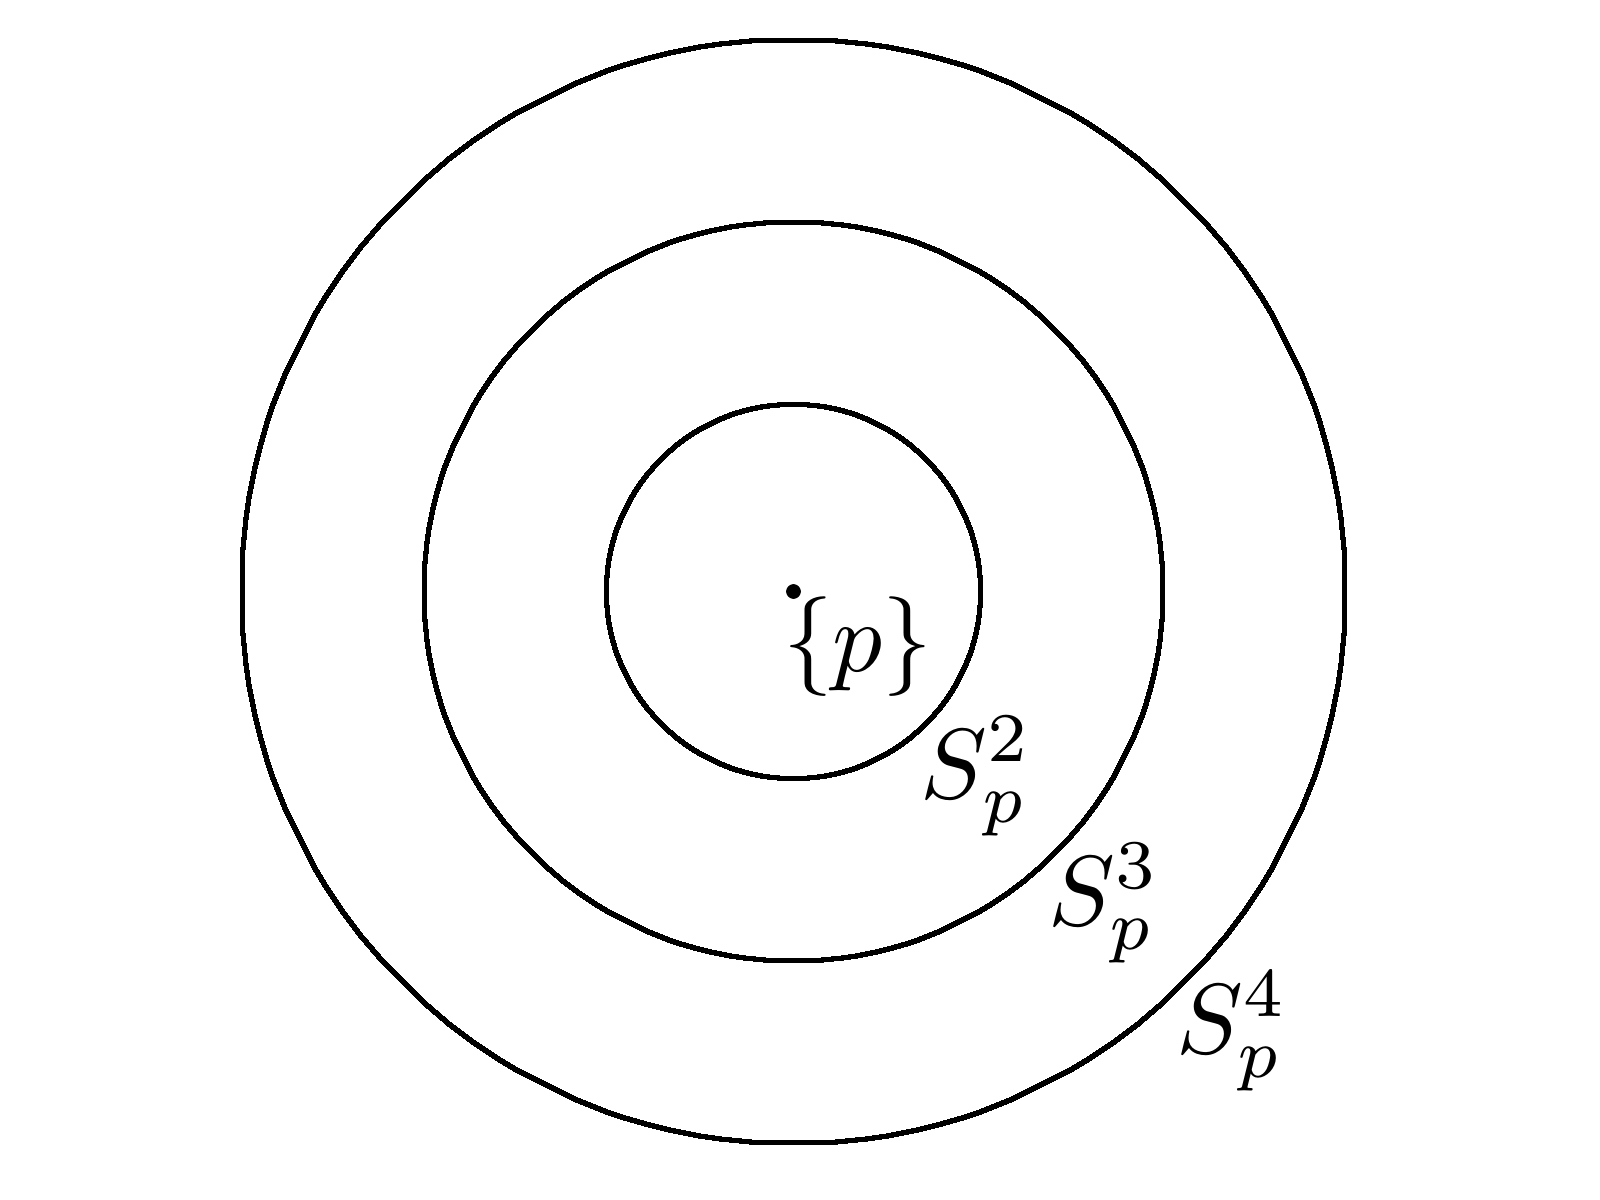
\includegraphics[width=\textwidth]{Similarityspheres.png}
	\caption{A two-dimensional representation of $n$-dimensional conceptual similarity spheres for a simple language with 4 equivalence classes\label{fig:spheres}}
\end{figure}

Since these sets are defined over a conceptual similarity relation relative to a sentence relative to language and a probability function, these might be called conceptual similarity spheres and bear \i{some} structural resemblance to the similarity spheres used for counterfactual semantics by \textcite{Lewis1973-LEWC-2}. Most notable differences are that (a) the subjects of discourse here aren't possible worlds at all and instead sentences of a language and (b) that this is not an objective ordering of any kind and instead a purely subjective ordering based on an agent's probability function. Given such a probability function, however, the ordering is rather fix. It would be interesting to investigate under which permutation of different measures the ordering stays invariant.

In short, through some simple structural features, a probability function yields a deep comparative notion of conceptual role of sentences and, One could presume, potentially some insights about meaning.

Next, we'll develop a simple example to see how this notion of conceptual role works.

\subsection{A Toy Example: The Lottery}

To use a familiar example, let's consider a standard fair $n$-ticket lottery scenario in which an agents has beliefs about a very narrow set of sentences $\{ t_1, \dots, t_n\}$, where $t_i$ is the sentence that the ticket number $i$ is the winning ticket. Assume a probability distribution of someone who is aware of the real chances involved, i.e.\ that the sentences describe disjoint events, such that $\Pr(t_1) = \cdots = \Pr(t_n) = \frac{1}{n}$ and, more importantly

\[
    \Pr(t_i \given t_j)  =
    \begin{cases*}
        1 & if $i = j$ \\
        0        & otherwise
    \end{cases*}
\]

We might, in this case, set $\mathfrak{c}(t_i, t_j) = \Pr(t_i \given t_j)$ and so with a euclidean distances measure 
\[
    \mathfrak{d}(t_i,t_j) = {\left( \sum_{k=1}^n {(t_{i_k}-t_{j_k})}^2 \right)}^{1/2} = \sqrt{2},  
\]
if $i \not = j$.

Hence, for any fixed $t_i$ there are only two corresponding similarity spheres:\footnote{No matter how we chose the similarity function $\mathfrak{s}$, as long as it is monotonously decreasing, as required above.} $S^1_{t_i} = \{ t_i\}$ and $S^2_{t_i}$, which contains all other sentences. 

This result isn't particularly exciting, but it serves well enough to indicate the spatial interpretation of conceptual role: Given no further information, $t_1$ and $t_{10}$ are just as close in meaning as $t_2$ and $t_{77}$. It is easy to see that were we to add additional constraints, such as that you yourself hold the ticket number 25 and we add the sentence $w$: ``I win the lottery!'', the previously strict symmetry is broken and $t_{25}$ takes a spatially distinguished position.

\subsection{Maybe Also Linda would be an interesting story?}
\subsection{Choosing a proper measure}

\section{Context Dependent Conceptual Role}

The whole enterprise of a spatial interpretation of a sentence is somewhat of a holistic approach, in that it evaluates meaning \i{globally} for a fixed language and agent. It is, however, pretty uncontroversial that the lexically same sentence can have different intended meanings, depending on the circumstances of when it's uttered. Relative to different context, the same words may mean something different. How can the presented account accommodate this? 

So far, there has been an implicit assumption that the conceptual role is represented relative to all of the probability function. This needn't be the case, though, and it is mathematically of course perfectly legitimate to restrict the sentences which make up the dimensions of our spatial interpretation. 

\textcite{Stalnaker1978-STAA-2} speaks of common ground amongst speakers in a conversation as establishing a context for utterances. This ground is determined by a context set, which consists in propositions assumed true for the purposes of a particular communication.

In a similar vein, we might adopt the notion of a context set populated with sentences instead of propositions as a means to restrict the spatial interpretation of meaning. Intuitively, this makes some sense: If we ask for a meaning in a particular context, and have already accepted the assumptions about the connection between meaning and evidential relation described in this paper, it is quite natural to restrict the evidential relations that are interesting to us to to those that involve the particular context.

This needn't be just those sentences that correspond to propositions assumed true, but may be extended to sentences deemed \i{relevant} to the current interests. That relevance is commonly spelled out in terms of evidential relation makes this approach seem a bit circular, perhaps, but does not have to concern us now, as there are many ways to skin a cat, see below.

Intuitively, then, one way to work with a context is to ``chip away'' at the vector space and remove as many dimensions as needed such that only dimensions corresponding to a context set remain.

More formally, let $V$ be a vector space over $\mathbb{R}$ with dimensions corresponding to sentences in a language $\L$ as above, with an appropriate measure $\mathfrak{c}$ chosen. Let $C \subseteq \L$ fix a context set of sentences that interest us, and let $V_C$ be a vector space over $\mathbb{R}$ with dimensions corresponding to sentences in $C$.\footnote{Since $V$ is just $\mathbb{R}^n$, and $V_C$ is just $\mathbb{R}^m$ with $m \leqslant n$, it follows directly that $V_C$ is a subspace of $V$.} Then $V_C$ is a subspace of $V$.

In a subspace like this, the distances between sentences can, of course, change markedly compared to the surrounding space, since dimensions that made up the bulk of the distance could be disregarded. Each context, then, induces another family of orderings on $\L$ by conceptual similarity.

The metaphor of a context as a subspace has some interesting advantages. It could be interesting, for example, to compare the change in conceptual role of some expression \i{across} contexts. In what --- quantifiable --- sense is an expression used differently when uttered in another context? If $C$ and $D$ are such context sets, two sentences $p$ and $q \in \L$  (not necessarily in $C$ or $D$) may differ wildly in distance in conceptual similarity given $C$ vs.\ given $D$. 

Don't know where to go with the following, might be relegated to a footnote..

Since for two subspaces of $V$, say $V_C$ and $V_D$, $V_C \cup V_D$ as well as $V_C \cap V_D$ are subspaces of $V$, contexts can be combined at will. This might be interesting if we look at contexts from another angle: Given a sentence $p$, what are relevant other sentences? What could be considered a \i{total} context of $p$? Intuitively, those sentences that $p$ stands in an evidential relation with, or is not probabilistically independent of. Depending on the measure $\mathfrak{c}$ chosen, these might be exactly those sentences corresponding to the dimensions $p$ takes a non-zero value in $V$. This gives a total context set for $p$. Accordingly, this can be generated with additional sentences. The intersection of both yields the common context, another way to generate a subspace from a context set. 



\section{Inter-Personal Similarity of Conceptual Role}

So far, the spatial interpretation of conceptual role has only been developed for a single language, with a single probability function. What is really interesting, though, is whether the account can be extended so as to include inter-speaker similarity in conceptual role. This is a much needed notion, as it strives to deal with an explication of why communication between two speakers actually works, although they, let's plausibly assume, do not mean \i{exactly} the same when using linguistic expressions. 

The problem is, of course, quite notorious, and we can only hope to hint at a possible solution.

Intuitively, though, the answer seems clear: two speakers use their expression \i{similarly enough} for communication to properly function, exact sameness in meaning is not required. How does that figure in this account? Can we find a formal explication of this idea? We need to (i) find a measure for the similarity in conceptual role and (ii) explain what it means to be similarly enough that actual communication can take place.

{\color{red} (Perhaps briefly describe what field does and describe his problem)}

The simplest case assumes two agents with probability functions over the exact same language. It is now just a matter to slightly rewrite the previous results, carefully distinguishing between each agents probability function.

Suppose two speakers with languages $\L$ and $\L'$ and probability functions $\Pr$ and $\Pr'$, respectively.

\section{Linguistic Entities}
\section{Conceptual Learning}
\section{Objections, Conclusions and Future Research}
Symmetry and Transitivity can be problematic, see Gardenfors 2004 p. 112 and Lewis (p. 51)

Maybe problems with indexical expressions? Could be better to define the whole schose on possible worlds instead\ldots

p and q can be on the same semantic location but be different sentences
\section{Replace Meaning with Conceptual Role}
\nocite{*}
\printbibliography{}
\end{document}
